\documentclass[UTF8, 11pt, a4paper]{ctexart}
\usepackage{tikz}
\begin{document}

% starts from (x,y)
% with center (x-r*cos(start), y-r*sin(start)) and

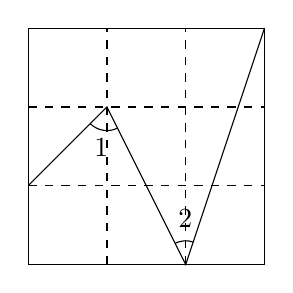
\begin{tikzpicture}
\draw (0,0)--(3,0)--(3,3)--(0,3)--cycle;
\draw[dashed](1,0)--(1,3) (2,0)--(2,3) (0,1)--(3,1) (0,2)--(3,2);
\draw (0,1)--(1,2) --(2,0)--(3,3);

% arctan(2)=63.43494882
\coordinate (P12) at (1, 2);
% r=0.3; r*cos(225)=-0.212; r*sin(225)=-0.212
\coordinate (start_1) at ([shift={(-0.212, -0.212)}] P12);
\draw(start_1) arc (225:297:0.3);

% arctan(3)=71.56505118
% r = 0.3; r*cos(71.565)=0.095; r*sin(71.565)=0.285
\coordinate (P20) at (2, 0);
\coordinate (start_2) at ([shift={(0.095, 0.285)}] P20);
% 180-63.435=116.565
\draw(start_2) arc (71.565:116.565:0.3);

\node at ([shift={(0.14,-0.3)}] start_1) {1};
\node at ([shift={(-0.1,0.3)}] start_2) {2};

\end{tikzpicture}

\end{document}